%%This is a very basic article template.
%%There is just one section and two subsections.
\documentclass[english,a4paper]{scrartcl}

\usepackage{graphicx}
\usepackage{listings}
\usepackage{color}
\usepackage{makeidx}
\usepackage{hyperref}
\usepackage{parskip}
\usepackage{multirow}
\usepackage{tocloft}
\renewcommand{\cftsecaftersnumb}{\hspace{6em}}
\renewcommand{\cftsubsecaftersnumb}{\hspace{6em}}
\renewcommand{\cftsubsubsecaftersnumb}{\hspace{6em}}

\makeindex

\hypersetup{
    %bookmarks=true,         % show bookmarks bar?
    unicode=false,          % non-Latin characters in Acrobat’s bookmarks
    pdftoolbar=true,        % show Acrobat’s toolbar?
    pdfmenubar=true,        % show Acrobat’s menu?
    pdffitwindow=false,     % window fit to page when opened
    pdfstartview={FitH},    % fits the width of the page to the window
    pdftitle={TDT4205 Compilers - Exercise 4 - hvatum},    % title
    pdfauthor={Stian Hvatum},     % author
    pdfsubject={TDT4205 Compilers},   % subject of the document
    pdfcreator={Stian Hvatum},   % creator of the document
    pdfproducer={Stian Hvatum}, % producer of the document
    pdfnewwindow=true,      % links in new window
    colorlinks,       % false: boxed links; true: colored links
    linkcolor=black,          % color of internal links
    citecolor=green,        % color of links to bibliography
    filecolor=magenta,      % color of file links
    urlcolor=cyan           % color of external links
}

\lstset{ %
  literate= {+}{{$+$}}1 {*}{{$*$}}1 {=}{{$\gets$}}1 
            {<=}{{$\leq$}}1 {>=}{{$\geq$}}1 {!=}{{$\neq$}}1 
            {==}{{$\equiv$}}1 {=>}{{$\leadsto$}}1
            {->}{{$\rightarrow$}}1
}

\definecolor{listinggray}{gray}{0.9}
\definecolor{lbcolor}{rgb}{0.9,0.9,0.9}
\lstset{
    keywordstyle=\bfseries\ttfamily\color[rgb]{0,0,1},
    identifierstyle=\ttfamily,
    commentstyle=\color[rgb]{0.133,0.545,0.133},
    stringstyle=\ttfamily\color[rgb]{0.627,0.126,0.941},
    showstringspaces=false,
    basicstyle=\tiny,
    numberstyle=\tiny,
    framexleftmargin=3pt,
    numbers=left,
    stepnumber=1,
    numbersep=15pt,
    tabsize=2,
    breaklines=true,
    prebreak = \raisebox{0ex}[0ex][0ex]{\ensuremath{\hookleftarrow}},
    breakatwhitespace=false,
    aboveskip={1.5\baselineskip},
    columns=fixed,
    upquote=true,
    extendedchars=true,
  	frame=l,
    sensitive=true,
}

\renewcommand{\thesection}{PART \arabic{section}}
\renewcommand{\thesubsection}{Task \arabic{section}.\arabic{subsection}}
\renewcommand{\thesubsubsection}{\arabic{subsubsection}.}

\title{TDT4205 Compilers\\
\Huge Exercise 4}
\author{Stian Hvatum (hvatum)\\MTDT}

\begin{document}
\maketitle
\tableofcontents
\section{Theory and Assembly Programming}
\subsection{Stack Frames}
\subsubsection{What is a stack frame}
A \emph{stack frame} is a location in a programs logical memory, or more
precicely, on the \emph{stack}, where it keeps the current local variables. The stack
frame grows as local variables are added, and shrinks as they are poped of, eg.
if they are not going to be used any more.

\subsubsection{Stack frame illustration}
\centerline{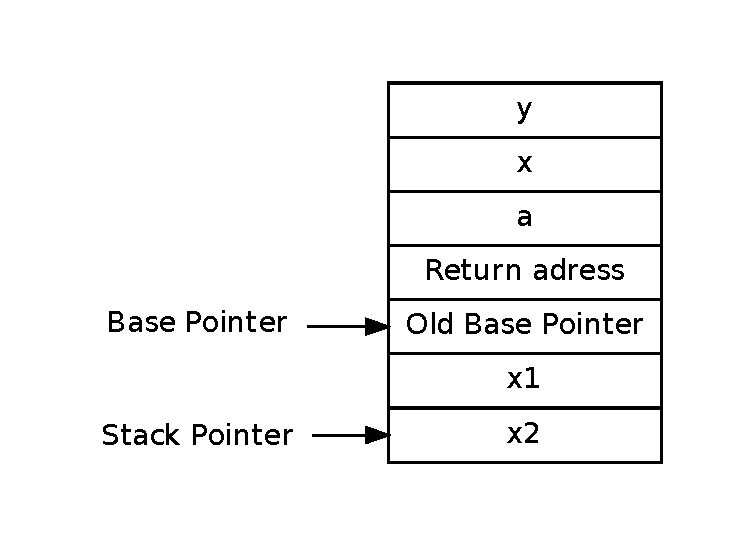
\includegraphics[width=300px]{stackframe.pdf}}
\subsubsection{Setting up and tearing down stack frames}

\newpage
\subsection{x86 Assembly Programming}
The complete file \emph{foo.s} is attached with the delivery of this file.
\begin{lstlisting}[language={[x86masm]Assembler}]
foo:
    /* Store old base pointer on top of stack */
    pushl   %ebp

    /* Set new stack base (ebp) to old top-of-stack (esp) */
    movl    %esp, %ebp

    /* Store 0 in ecx  (loop starts at 1, but is incremented in first test) */
    movl    $0,   %ecx

    /* Store 0 on the stack, our sum value */
    pushl   $0

    /* And start loop-test */
    jmp tst_lp

lbody:
    /* Loop body */
    /* Modulo = divide and check rest-register */


    /* Check for input divisible by 3 */
    movl    %ecx, %eax
    movl    $3,   %ebx
    cdq
    idiv    %ebx
    /* edx now contains ecx mod 3 */
    cmp     $0,   %edx
    jz tst_ok /* Test true */

     /* Check for input divisible by 5 */
    movl    %ecx, %eax
    movl    $5,   %ebx
    cdq
    idiv    %ebx
    /* edx now contains ebx mod 5 */
    cmp     $0,   %edx
    jnz tst_lp /* Test false */
tst_ok:
    addl    %ecx, -4(%ebp)
    
tst_lp:
    /* Get the function argument and store in ebx */
    movl    8(%ebp), %ebx

   /* Increment and test */ 
    inc %ecx
    /* if ebx < ecx => jump to start of loop */
    cmp %ebx, %ecx
    jl lbody

    pushl -4(%ebp)
    /* Print results */
    /* sum is on top of stack */
    pushl   $.STRING0
    call    printf

    /* Clean up on stack */
    addl    $8, %esp
    /* Clean up stack frame */
    leave

    /* Return home */
    ret
\end{lstlisting}
\newpage
\subsection{Symbol Tables}
\subsubsection{Stack offset}
\begin{description}
\item[a] -4
\item[b] -8
\item[c] $-28 (-8 - (4 \cdot 5))$
\end{description}

\subsubsection{Lexical depth}


\printindex
\end{document}
